\begin{examplebox}
\textbf{\textcolor{CExample}{例 1｜先会看图：普通闭区间（基础）}}

\textbf{题目：}已知 $f(x)=2x^2-8x+3$，求其在 $[1,4]$ 上的最小值和最大值。

\textbf{解：}配方得 $f(x)=2(x-2)^2-5$，对称轴 $x=2$，开口向上；$2\in[1,4]$，所以最小值为 $f(2)=-5$。端点到轴距离分别为 $|1-2|=1$ 和 $|4-2|=2$，右端更远，所以最大值为 $f(4)=3$（左端 $f(1)=-3$）。
\begin{center}
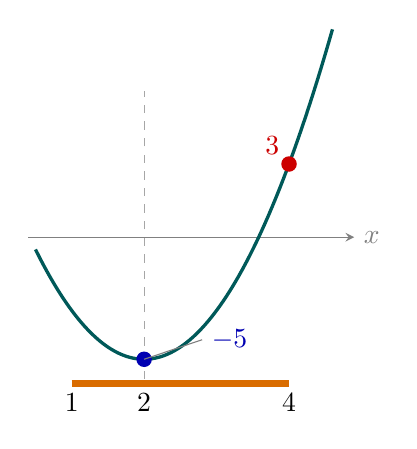
\begin{tikzpicture}[x=0.92cm,y=0.31cm,>=stealth]
 \draw[->,gray] (0.4,0)--(4.9,0) node[right] {$x$};
 \draw[dashed,gray!70] (2,-5.8)--(2,6);
 \draw[very thick,teal!70!black,domain=0.5:4.6,samples=80] plot (\x,{2*(\x-2)^2-5});
 \draw[line width=2.5pt,orange!85!black] (1,-6)--(4,-6);
 \fill[blue!70!black] (2,-5) circle (2.8pt) ;\draw[gray] (2,-5)--(2.8,-4.2) node[right,blue!70!black] {$-5$};
 \fill[red!80!black] (4,3) circle (2.8pt) node[above left] {$3$};
 \node[below] at (1,-6) {$1$}; \node[below] at (2,-6) {$2$}; \node[below] at (4,-6) {$4$};
\end{tikzpicture}

\end{center}
\textbf{答案：}$\boxed{f_{\min}=-5,\quad f_{\max}=3}$。\textit{做得快的原因：最高点直接找离轴远的端点，不必逐个比较函数值。}

\medskip
\textbf{\textcolor{CExample}{例 2｜最重要：区间移动，最大最小都求（提高）}}

\textbf{题目：}函数 $f(x)=(x-2)^2$ 不动，区间 $[t,t+2]$ 左右移动。用 $t$ 表示这段区间上的最大值、最小值。

\textbf{第一步（最小值看“有没有碰轴”）：}轴是 $x=2$。
\begin{itemize}[leftmargin=*,itemsep=0.23em]
 \item $t+2<2$（即 $t<0$）：区间在轴左，右端较近，$f_{\min}=f(t+2)=t^2$；
 \item $t\le2\le t+2$（即 $0\le t\le2$）：区间包含轴，$f_{\min}=f(2)=0$；
 \item $t>2$：区间在轴右，左端较近，$f_{\min}=f(t)=(t-2)^2$。
\end{itemize}
\[
 \boxed{f_{\min}(t)=
 \begin{cases}
 t^2,&t<0,\\ 0,&0\le t\le2,\\ (t-2)^2,&t>2.
 \end{cases}}
\]
\textbf{第二步（最大值看“端点谁更远”）：}区间中点是 $t+1$。令 $t+1=2$，得到\textbf{分界点 $t=1$}。
\begin{itemize}[leftmargin=*,itemsep=0.23em]
 \item $t<1$：左端点 $t$ 更远，$f_{\max}=f(t)=(t-2)^2$；
 \item $t>1$：右端点 $t+2$ 更远，$f_{\max}=f(t+2)=t^2$；
 \item $t=1$：两端都离轴 $1$ 格，$f(1)=f(3)=1$。
\end{itemize}
\[
 \boxed{f_{\max}(t)=
 \begin{cases}
 (t-2)^2,&t<1,\\ t^2,&t\ge1.
 \end{cases}}
\]
\textbf{边界说明：}在 $t=1$ 两式都等于 $1$，没有冲突；分段也可写成 $t<1$、$t\ge1$。
\begin{center}
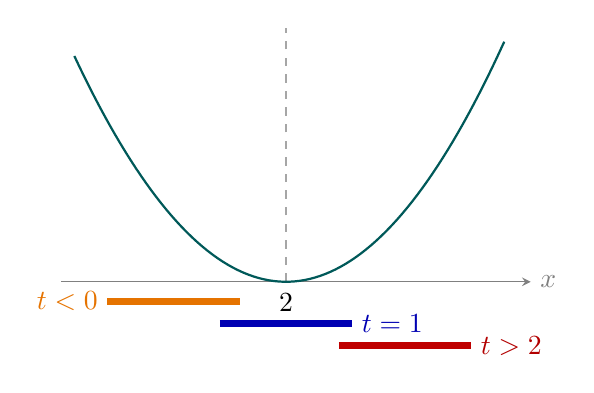
\begin{tikzpicture}[x=0.84cm,y=0.28cm,>=stealth]
 \draw[->,gray] (-1.4,0)--(5.7,0) node[right] {$x$};
 \draw[dashed,gray!70] (2,0)--(2,11.5);
 \draw[thick,teal!70!black,domain=-1.2:5.3,samples=85] plot (\x,{(\x-2)^2});
 \draw[line width=2.6pt,orange!90!black] (-0.7,-0.9)--(1.3,-0.9);
 \draw[line width=2.6pt,blue!70!black] (1,-1.9)--(3,-1.9);
 \draw[line width=2.6pt,red!75!black] (2.8,-2.9)--(4.8,-2.9);
 \node[left,orange!90!black] at (-0.7,-0.9) {$t<0$};
 \node[right,blue!70!black] at (3,-1.9) {$t=1$};
 \node[right,red!70!black] at (4.8,-2.9) {$t>2$};
 \node[below] at (2,-0.1) {$2$};
\end{tikzpicture}

\end{center}
\textbf{答案要点：}最小值的分界点为 $t=0,2$（\textbf{端点碰轴}）；最大值的分界点为 $t=1$（\textbf{中点碰轴}）。\textbf{不要把两类分界点混成一类。}

\medskip
\textbf{\textcolor{CExample}{例 3｜倒过来的抛物线（巩固）}}

\textbf{题目：}已知 $g(x)=-x^2+4x-1$，在 $[t,t+2]$（$t\in\mathbb R$）上的最大值是多少？

\textbf{解：}$g(x)=-(x-2)^2+3$，轴还是 $x=2$，但\textbf{开口向下，最高点在轴上}。
\begin{itemize}[leftmargin=*,itemsep=0.23em]
 \item $t<0$：区间在轴左，右端更近，$g_{\max}=g(t+2)=3-t^2$；
 \item $0\le t\le2$：区间包含轴，$g_{\max}=g(2)=3$；
 \item $t>2$：区间在轴右，左端更近，$g_{\max}=g(t)=3-(t-2)^2$。
\end{itemize}
\[
 \boxed{g_{\max}(t)=
 \begin{cases}
 3-t^2,&t<0,\\ 3,&0\le t\le2,\\ 3-(t-2)^2,&t>2.
 \end{cases}}
\]
\begin{center}
\begin{tikzpicture}[x=0.92cm,y=0.32cm,>=stealth]
 \draw[->,gray] (-0.5,0)--(4.65,0) node[right] {$x$};
 \draw[dashed,gray!70] (2,-4.5)--(2,3.7);
 \draw[very thick,teal!70!black,domain=-0.3:4.5,samples=75] plot (\x,{3-(\x-2)^2});
 \draw[line width=2.5pt,orange!85!black] (1,-4)--(3,-4);
 \fill[red!80!black] (2,3) circle (2.7pt) node[above right] {最高点 $3$};
 \node[below] at (1,-4) {$t=1$}; \node[below] at (3,-4) {$t+2=3$};
 \node[below] at (2,-0.2) {$2$};
\end{tikzpicture}

\end{center}
\textbf{关键：}不必重记一套，\textbf{把开口向上时的“最低”换成“最高”}即可。

\medskip
\textbf{\textcolor{CExample}{例 4｜已知最小值，反求区间（应用）}}

\textbf{题目：}已知 $p(x)=x^2-2x+2$ 在 $[s,s+2]$ 上的最小值是 $3$，求 $s$。

\textbf{解：}$p(x)=(x-1)^2+1$，轴 $x=1$，最低点函数值为 $1$。题目说区间内最小值是 $3$，说明\textbf{区间不能包含轴}（否则最小值只能是 $1$）。
\begin{itemize}[leftmargin=*,itemsep=0.25em]
 \item 区间在轴右：$s>1$，最近端点为 $s$。$(s-1)^2+1=3\Rightarrow s=1\pm\sqrt2$，结合 $s>1$，取 $s=1+\sqrt2$。
 \item 区间在轴左：$s+2<1$，最近端点为 $s+2$。$(s+1)^2+1=3\Rightarrow s=-1\pm\sqrt2$，结合 $s<-1$，取 $s=-1-\sqrt2$。
\end{itemize}
\begin{center}
\begin{tikzpicture}[x=0.89cm,y=0.29cm,>=stealth]
 \draw[->,gray] (-3.2,0)--(5.1,0) node[right] {$x$};
 \draw[dashed,gray!70] (1,0)--(1,13.2);
 \draw[very thick,teal!75!black,domain=-2.8:4.8,samples=85] plot (\x,{(\x-1)^2+1});
 \draw[line width=2.5pt,orange!90!black] (-2.4,-0.58)--(-0.4,-0.58);
 \draw[line width=2.5pt,blue!75!black] (2.4,-1.45)--(4.4,-1.45);
 \node[below,orange!85!black] at (-1.3,-0.58) {区间在左};
 \node[below,blue!75!black] at (3.4,-1.45) {区间在右};
 \node[below] at (1,-0.1) {$1$};
 \fill[blue!75!black] (-0.41421356,3) circle (2.5pt) node[above right] {$3$};
 \fill[blue!75!black] (2.41421356,3) circle (2.5pt) node[above left] {$3$};
 \fill[red!75!black] (1,1) circle (2.4pt) node[above right] {顶点值 $1$};
\end{tikzpicture}

\end{center}
\textbf{答案：}$\boxed{s=1+\sqrt2\ \text{或}\ s=-1-\sqrt2}$。\textbf{检查：}这两个 $s$ 对应的区间都不含 $1$，且近轴端点处的函数值都是 $3$。
\end{examplebox}
